\section{Nguồn web, PDF và truy vết căn cứ}
\subsection{Tài liệu được bổ sung}
Bản cập nhật bổ sung 12 đoạn: sáu đoạn từ PDF NIDDK, hai đoạn từ trang Healthy Living with Diabetes và bốn đoạn từ hai bài Vinmec. Tổng KB gồm 58 đoạn tham chiếu 22 nguồn. Nguồn tiếng Việt được chọn là các bài dinh dưỡng và chăm sóc bàn chân của hệ thống y tế Vinmec. Các đoạn bổ sung giới hạn ở tự chăm sóc và chuẩn bị trao đổi với nhân viên y tế.

\begin{longtable}{p{3cm}p{6.5cm}p{4.3cm}}\caption{Bản nguồn được lưu và phạm vi trích xuất.}\\\toprule Nguồn & Nội dung & Định vị\\\midrule\endfirsthead\toprule Nguồn & Nội dung & Định vị\\\midrule\endhead
NIDDK PDF & Guiding Principles for the Care of People with or at Risk for Diabetes: tự chăm sóc, mục tiêu, dinh dưỡng và ví dụ vận động. & Trang vật lý 27, 28, 31, 32, 34.\\
NIDDK web & Khẩu phần, kế hoạch bữa ăn và lưu ý khi bỏ hoặc trễ bữa với một số thuốc. & Mục Plan what to eat or drink và Plan how much to eat or drink.\\
Vinmec & Chế độ dinh dưỡng cho người tiểu đường; cách chăm sóc bàn chân. & Tiêu đề mục, URL và trích dẫn ngắn.\\\bottomrule\end{longtable}

PDF và văn bản web NIDDK được lưu trong \path{data/source_documents/}. Với Vinmec, project giữ trích dẫn ngắn và bản tóm tắt, không phân phối lại toàn bài. Tệp \path{data/source_curation.json} ghi nội dung biên soạn cùng vị trí đối chiếu. Script \path{scripts/build_sourced_kb.py} đọc các bản nguồn local, kiểm tra trích dẫn, số trang và SHA-256 rồi dựng \path{data/knowledge_curated.json}; script này không gọi mạng hay mô hình ngôn ngữ.

PDF là tài liệu lưu trữ có các tham chiếu từ giai đoạn trước. Bản cập nhật chỉ chọn những nguyên tắc tự chăm sóc trong các trang đã nêu, không dùng tài liệu này để thay ngưỡng chẩn đoán hiện hành hoặc chỉ định liều. Việc đối chiếu trích đoạn và mã băm chứng minh nguồn gốc dữ liệu, chưa chứng minh chất lượng chuyên môn của mọi bản tóm tắt.

\subsection{Đưa tài liệu vào KG và RAG}
Sau khi hợp nhất ba tệp KB, chỉ mục TF-IDF được xây lại. Các bộ ba mới được nạp bằng MERGE; Neo4j có 169 khái niệm và 106 quan hệ. Quan hệ của tài liệu bổ sung giữ thêm tệp nguồn, SHA-256 và số trang nếu là PDF. Bộ xuất bảo toàn các trường đó, đồng thời đóng gói bản nguồn để có thể kiểm tra lại.

Khi câu hỏi chỉ rõ Vinmec hoặc PDF, truy xuất giới hạn kết quả theo nguồn được yêu cầu. Việc chuẩn hóa tiếng Việt cần phân biệt cụm ``tài liệu'' với ``liều'' thuốc; trường hợp này được bổ sung vào kiểm tra định tuyến sau khi phát hiện một câu hỏi PDF bị chuyển nhầm sang nhánh thuốc. Các yêu cầu tính liều thật vẫn chịu luật an toàn trước truy xuất.

Liên kết PDF trên web mở bản lưu local qua \path{/api/source/}, kèm số trang. Người dùng có thể kiểm tra tài liệu mà không cần Internet. Việc thu thập nguồn công khai lúc xây KB có truy cập web theo yêu cầu; luồng hội thoại sau đó không tự tải tài liệu hoặc gửi dữ liệu sức khỏe tới dịch vụ ngoài.

\section{Hai vai trò agent sau kết quả mô hình}
\subsection{Nhận xét và hỗ trợ có nguồn}
Agent Nhận xét mô hình nhận đầu ra MLP và giải thích ý nghĩa nhãn hoặc điểm, phép đo trên test và giới hạn sử dụng. Agent Hỗ trợ người dùng nhận bản nhận xét cùng tài liệu đã truy xuất, trả ba mục: ăn uống, theo dõi bữa ăn và thuốc, chuẩn bị trao đổi khi đi khám. Mỗi mục có mã nguồn riêng. Đây là các bước hỗ trợ chung; nhãn tổng hợp và điểm tiến triển không được dùng để tính chế độ ăn hoặc xác nhận bệnh.

Hai vai trò này có handler thật trong \path{app/model_support.py} và trao đổi qua MessageBus. Khi người dùng bấm ``Nhận xét và hỗ trợ'', trình duyệt chuyển mẫu nghiên cứu sang chat và hiển thị thông báo ngữ cảnh. Các lượt hỏi tiếp có thể đính kèm mẫu; backend tự tính lại đầu ra từ các trường, không nhận một kết luận do trình duyệt tự gán. Nút ``Bỏ ngữ cảnh mẫu'' hoặc ``Cuộc trò chuyện mới'' xóa ngữ cảnh cho các lượt sau. Nếu người dùng mô tả tình huống nguy hiểm, nhánh an toàn trả trước bước mô hình và truy xuất.

\begin{figure}[p]\centering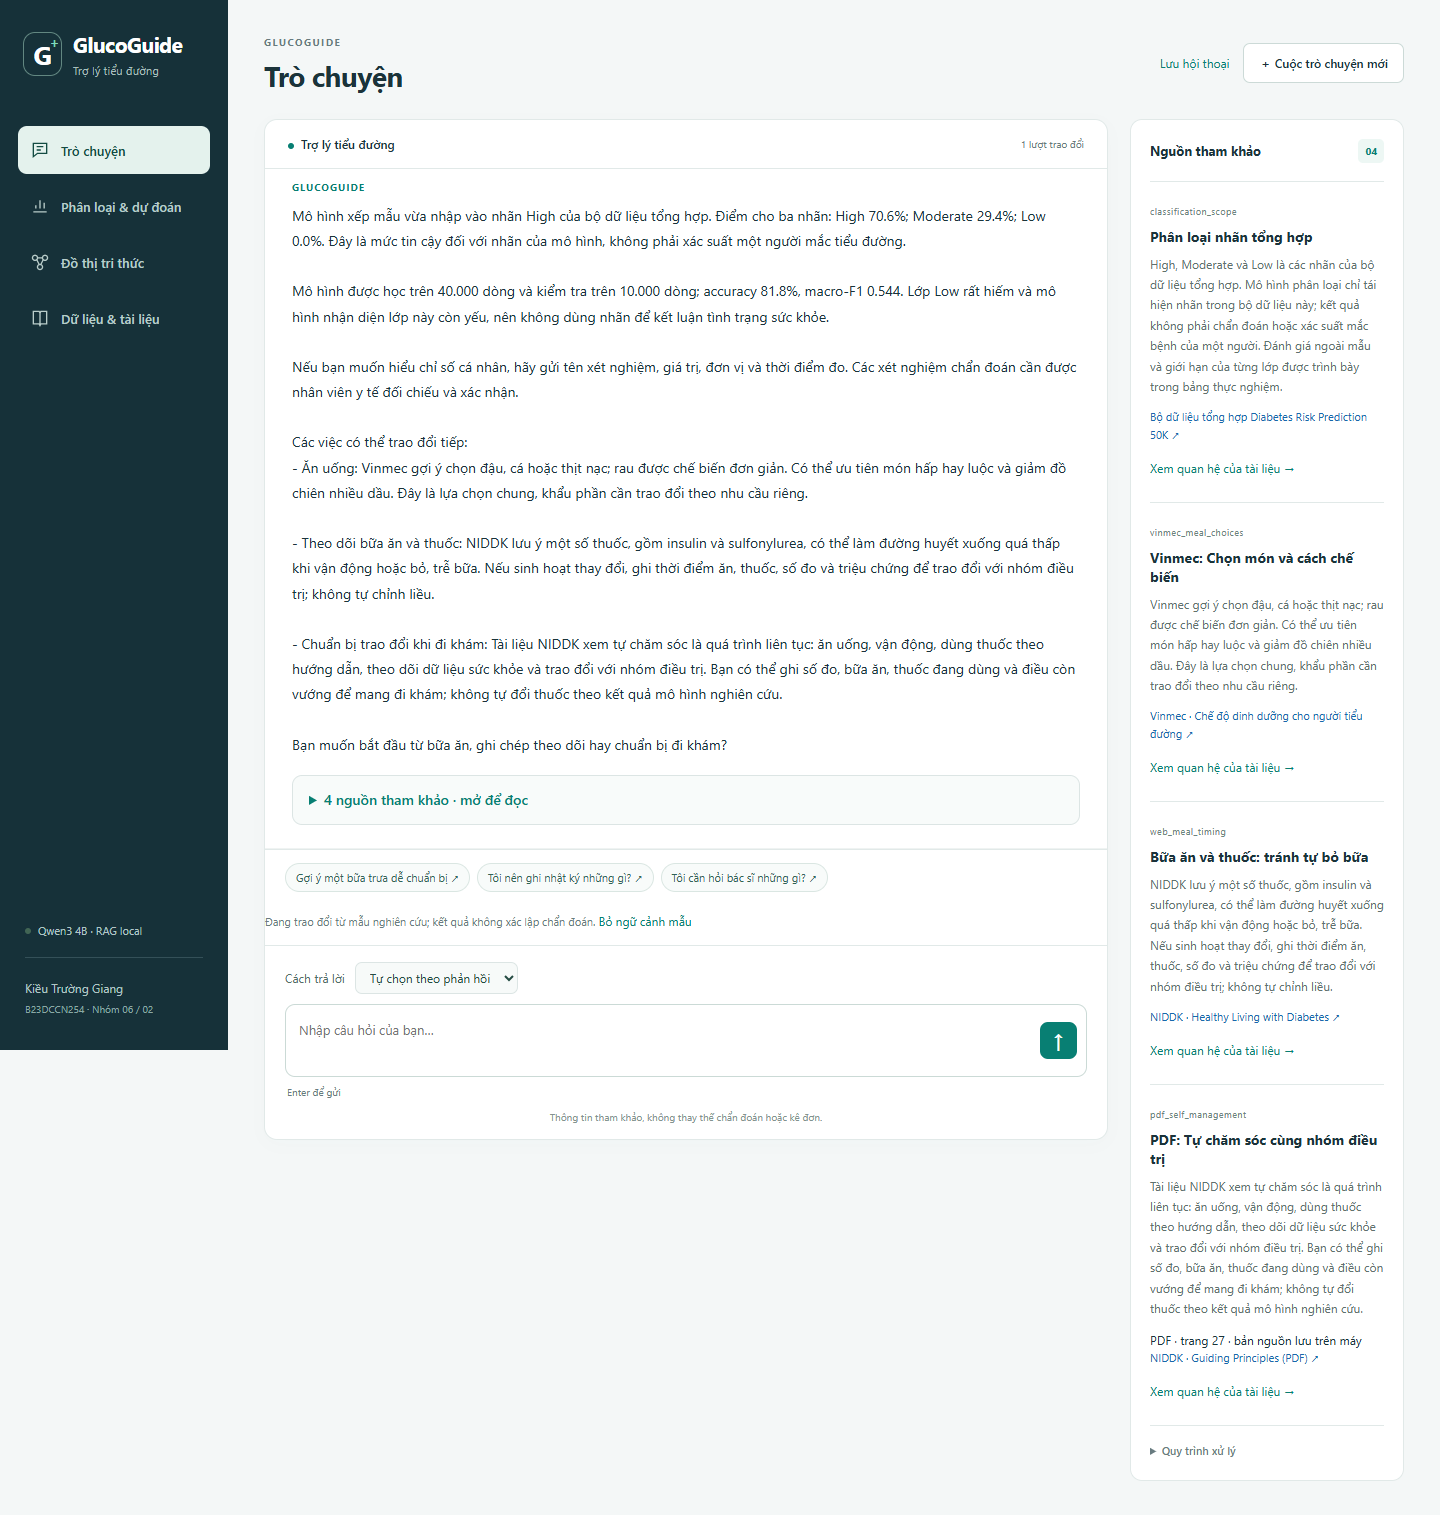
\includegraphics[width=\linewidth,height=.81\textheight,keepaspectratio]{demo-model-support.png}\caption{Kết quả mô hình được chuyển sang trợ lý với ba mục hỗ trợ có nguồn và thông báo ngữ cảnh nghiên cứu.}\end{figure}
\begin{figure}[p]\centering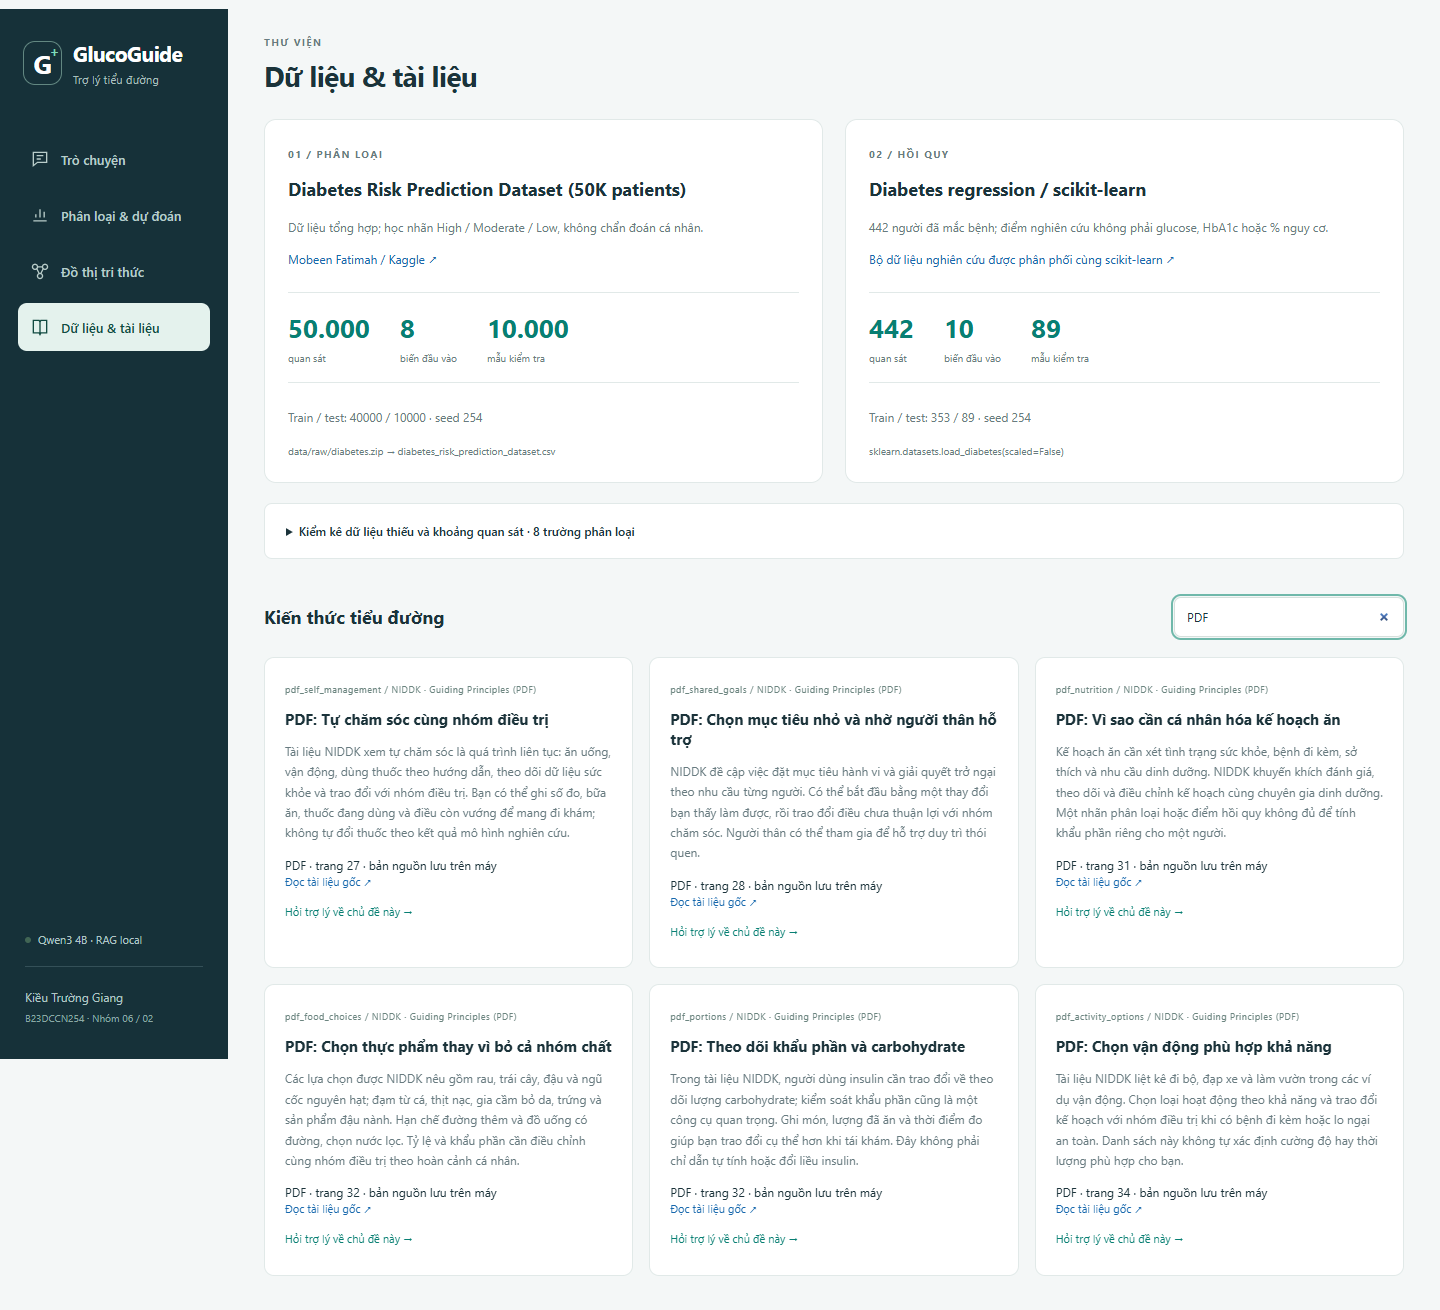
\includegraphics[width=\linewidth,height=.81\textheight,keepaspectratio]{demo-pdf-sources.png}\caption{Tra cứu sáu đoạn PDF trên web; mỗi đoạn có liên kết mở bản nguồn local tại trang tương ứng.}\end{figure}
\clearpage

\subsection{Kiểm thử và phạm vi kết luận}
Kiểm tra nguồn và hỗ trợ gồm 13 điều kiện: trích đoạn, trang PDF, mã băm, hai bài toán mô hình, ba mục có nguồn, hỏi tiếp, xóa ngữ cảnh, kiểm tra đầu vào và ưu tiên cấp cứu. Tám kiểm tra giao diện xác nhận đường đi từ form tới chat, liên kết PDF và các request chỉ tới máy local. Kết quả nằm tại \path{results/sources_support_tests.json} và \path{results/support_ui_tests.json}.

Tập hồi quy truy xuất 22 câu giữ nguyên tài liệu kỳ vọng trước khi mở rộng KB: Hit@1 đạt 85\%, Hit@4 đạt 100\%, MRR@4 đạt 0,917. Một số đoạn mới cạnh tranh vị trí đầu với đoạn cũ, nên Hit@1 giảm so với bản trước dù vẫn tìm thấy căn cứ kỳ vọng trong bốn vị trí đầu. Tập tám câu kiểm tra nguồn PDF/Vinmec được lưu riêng trong \path{data/rag_source_evaluation.json}; sau khi sửa lỗi định tuyến ``tài liệu'', cả tám tìm đúng tài liệu ở vị trí đầu. Các phép đo này kiểm tra truy xuất và luồng phần mềm, không đo độ chính xác chẩn đoán hoặc hiệu quả tư vấn cho bệnh nhân thật.
